\documentclass{VUMIFPSkursinis}
\usepackage{algorithmicx}
\usepackage{algorithm}
\usepackage{algpseudocode}
\usepackage{amsfonts}
\usepackage{amsmath}
\usepackage{bm}
\usepackage{caption}
\usepackage{color}
\usepackage{float}
\usepackage{graphicx}
\usepackage{listings}
\usepackage{subfig}
\usepackage{wrapfig}
\usepackage{longtable}
\usepackage{tabularx}
\usepackage{tabu}
\usepackage{multirow}
\usepackage{rotating}
\usepackage[table]{xcolor}

\usepackage{datatool}% http://ctan.org/pkg/datatool
\newcommand{\sortitem}[2][\relax]{%
  \DTLnewrow{list}% Create a new entry
  \ifx#1\relax
    \DTLnewdbentry{list}{sortlabel}{#2}% Add entry sortlabel (no optional argument)
  \else
    \DTLnewdbentry{list}{sortlabel}{#1}% Add entry sortlabel (optional argument)
  \fi%
  \DTLnewdbentry{list}{description}{#2}% Add entry description
}
\newenvironment{sortedlist}{%
  \DTLifdbexists{list}{\DTLcleardb{list}}{\DTLnewdb{list}}% Create new/discard old list
}{%
  \DTLsort{sortlabel}{list}% Sort list
  \begin{itemize}%
    \DTLforeach*{list}{\theDesc=description}{%
      \item \theDesc}% Print each item
  \end{itemize}%
}

% Titulinio aprašas
\university{Vilniaus universitetas}
\faculty{Matematikos ir informatikos fakultetas}
\department{Programų sistemų katedra}
\papertype{Laboratorinis darbas}
\title{Festivalių informacinė sistema}
\titleineng{}
\status{2 kurso 5 grupės studentai}
\author{Mantas Petrikas}
\secondauthor{Olga Joana Šimitaitė}   % Pridėti antrą autorių
\thirdauthor{Miglė Vaitulevičiūtė}   % Pridėti trečią autorių
\fourthauthor{Vytautas Žilinas}   % Pridėti ketvirtą autorių
\supervisor{Vytautas Valaitis}
\date{Vilnius – \the\year}

% Nustatymai
\setmainfont{Palemonas}   % Pakeisti teksto šriftą į Palemonas (turi būti įdiegtas sistemoje)
\bibliography{bibliografija}

\definecolor{light-gray}{gray}{0.8}

\begin{document}
\maketitle

\tableofcontents

\sectionnonum{Įvadas}
Lietuvoje vyksta daug festivalių, kurie savo informacija skelbia atskirose vietose, tačiau nėra patogios naudotis informacinės sistemos. 
Todėl atsižvelgę į tai nusprendėme, kad geriausia būtų sukurti tinklalapį, kuriame vartotojas galėtų lengvai bei efektyviai atrasti jį dominančią informacija apie Lietuvoje vykstančius festivalius, taip padidinant žmonių susidomėjimą Lietuvos festivaliais bei prisidedant prie jų garsinimo.

Šio, antro laboratorinio darbo tikslas yra suformuluoti vartotojo interfeiso, funkcinius ir nefunkcinius reikalavimus.
\section{Sistemos reikalavimai}
Šiame skyriuje pateikiami vartotojo interfeiso, funkciniai ir nefunkciniais reikalavimai.
\subsection{Vartotojo interfeiso reikalavimai}
Šiame poskyriuje pateikiami metaforos reikalavimai, formuluojamos užduotys, užduočių formulavimo kalbos reilkalavimai, užduočių formulavimo protokolo reikalavimai, interfeiso darnos ir standartizavimo reikalavimai, pranešimų formulavimo reikalavimai ir interfeiso individualizavimo reikalavimai. 

\centerline{1 lentelė. Sistemos vartotojo interfeiso reikalavimai} 
\setlength\tabcolsep{4pt}
\begin{longtable}{|p{1cm}|p{3cm}|p{9cm}|c|}
\hline
Tipas & Numeris & Aprašymas & Būtinumas \\ \hline
\endfirsthead
\hline
Tipas & Numeris & Aprašymas & Būtinumas \\ \hline
\endhead
\hline
\endfoot
\hline
\multirow{84}{*}{\rotatebox{90}{~~~~~~~~~~~~~~~~~~~~~~~~~~~~~~~~~~~~~~~~~~~~~~~~~~~~~~~~~~~~~~~~~~~~~~~~~~~~~~~~~~~~~~~~~~~~~~~~~~~~~~~~~~~~~~~~~~~~~~~~~~~~~~~~~~~~~~~~~~~~~~~~~~~~~~~~~~~~~~~~~~~~~~~~~~~~~~~~~~~~~~~~~~~~~~~~~~~~~~~~~~~~~~~~~~~~~~~~~~~~~~~~~~~~~~~~~~~~~~~~~~~~~~~~~~~~~~~~~~~~~~~~~~~~~~~~~~~~~~~~~~~~~~~~~~Vartotojo interfeiso reikalavimai}} & IR.1 \cellcolor{light-gray}& \multicolumn{2}{l|}{ \cellcolor{light-gray}Dalykinės srities metaforų reikalavimai} \\ \cline{2-4} 
 & IR.1.1 & Nuo puslapio viršaus navigacijos įrankių juosta & Būtina \\ \cline{2-4} 
 & IR.1.2 & Nuoroda į festivalio informacijos puslapį vaizduojama kaip festivalio plakatas (paveikslėlis) & Būtina \\ \cline{2-4} 
 & IR.1.3 & "Mano meniu \textbackslash / išskleidžia prisijungusio vartotojo meniu (IR.4) & Būtina \\ \cline{2-4} 
 & IR.1.4 & "Mano meniu /\textbackslash ~suskleidžia prisijungusio vartotojo meniu (IR.4) & Būtina \\ \cline{2-4} 
 & IR 1.5 & Penkios žvaigždutės festivalio aprašymo puslapyje leidžia vertinti festivalį balais nuo vienio iki penkių. & Būtina \\ \cline{2-4} 
 & IR.1.6 & Nuotraukos ikona su apačioje esančiu užrašu "Nuotraukos" atidaro festivalio nuotraukų galeriją. & Būtina \\ \cline{2-4} 
 & IR.1.7 & "->" simbolis šalia nuotraukos leidžia eiti į prieš tai buvusią nuotrauką. & Būtina \\ \cline{2-4} 
 & IR.1.8 & "<-" simbolis šalia nuotraukos leidžia eiti į sekančią nuotrauką. & Būtina \\ \cline{2-4} 
 & IR.1.9 & Trikampis su viduje esančiu šauktuko ženklu (Priedas Nr.1)leidžia vartotojui pranešti apie netinkamą atsiliepimą ar komentarą . & Būtina \\ \cline{2-4} 
 &  \cellcolor{light-gray}IR.2 & \multicolumn{2}{l|}{ \cellcolor{light-gray}Vartotojo užduotių reikalavimai} \\ \cline{2-4} 
 & IR.2.1 & Susikurti savo paskyrą tinklalapyje. & Būtina \\ \cline{2-4} 
 & IR.2.2 & Sužinoti kokie yra naujausi festivaliai. & Būtina \\ \cline{2-4} 
 & IR.2.3 & Skaityti straipsnius apie festivalius. & Būtina \\ \cline{2-4} 
 & IR.2.4 & Gauti tikslią festivalio vietą. & Būtina \\ \cline{2-4} 
 & IR.2.5 & Gauti festivalio kainą ir nuorodą į oficialų bilietų pardavėjo tinklalapį. & Būtina \\ \cline{2-4} 
 & IR.2.6 & Gauti festivalio datą. & Būtina \\ \cline{2-4} 
 & IR.2.7 & Gauti festivalio aprašymą. & Būtina \\ \cline{2-4} 
 & IR.2.8 & Gauti oficialią festivalio tinklalapio nuorodą. & Būtina \\ \cline{2-4} 
 & IR.2.9 & Peržiūrėti konkretaus festivalio nuotraukas. & Būtina \\ \cline{2-4} 
 & IR.2.10 & Paremti mūsų tinklalapį. & Būtina \\ \cline{2-4} 
 & IR.2.11 & Diskutuoti su kitais vartotojais apie konkretų festivalį. & Būtina \\ \cline{2-4} 
 & IR.2.12 & Vertinti ir rašyti atsiliepimus apie festivalius. & Būtina \\ \cline{2-4} 
 & IR.2.13 & Susiplanuoti į kokius festivalius nori nuvykti. & Būtina \\ \cline{2-4} 
 & IR.2.14 & Pranešti apie netinkamus komentarus Diskusijų zonoje. & Būtina \\ \cline{2-4} 
 & IR.2.15 & Administratoriui gali palikti atsiliepimą apie tinklalapį. & Būtina \\ \cline{2-4} 
 & IR.2.16 & Peržiūrėti festivalių sąrašą. & Būtina \\ \cline{2-4} 
 & IR.2.17 & Sistemingai ieškoti norimo festivalio jų sąraše. & Būtina \\ \cline{2-4} 
 & IR.2.18 & Užsiprenumeruoti festivalį (gauti informaciją apie jį). & Būtina \\ \cline{2-4} 
 & IR.2.19 & Prisijungti prie savo paskyros. & Būtina \\ \cline{2-4} 
 &  \cellcolor{light-gray}IR.3 & \multicolumn{2}{l|}{ \cellcolor{light-gray}Administratorius užduotių reikalavimai} \\ \cline{2-4} 
 & IR.3.1 & Rasti konkretų vartotoją vartotojų sąraše. & Būtina \\ \cline{2-4} 
 & IR.3.2 & Priskirti vartotojui privilegijas (žurnalisto, administratoriaus ar paprasto vartotojo). & Būtina \\ \cline{2-4} 
 & IR.3.3 & Uždrausti prieiga tam tikram laikui. & Būtina \\ \cline{2-4} 
 & IR.3.4 & Ištrinti vartotoją. & Būtina \\ \cline{2-4} 
 & IR.3.5 & Redaguoti festivalio informaciją. & Būtina \\ \cline{2-4} 
 & IR.3.6 & Peržiūrėti festivalių sąrašą. & Būtina \\ \cline{2-4} 
 & IR.3.7 & Ieškoti tam tikro festivalio aprašymo. & Būtina \\ \cline{2-4} 
 & IR.3.8 & Patvirtinti informaciją apie naują festivalį. & Būtina \\ \cline{2-4} 
 & IR.3.9 & Taisyti festivalio informaciją. & Būtina \\ \cline{2-4} 
 & IR.3.10 & Peržiūrėti vartotojų atsiliepimus apie tinklalapį. & Būtina \\ \cline{2-4} 
 & IR.3.11 & Peržiūrėti vartotojų atsiliepimus apie festivalius. & Būtina \\ \cline{2-4} 
 & IR.3.12 & Filtruoti atsiliepimus pagal raktažodžius. & Būtina \\ \cline{2-4} 
 & IR.3.13 & Ištrinti netinkamus atsiliepimus. & Būtina \\ \cline{2-4} 
 & IR.3.14 & Peržiūrėti diskusijų žinutes. & Būtina \\ \cline{2-4} 
 & IR.3.15 & Filtruoti diskusijų žinutes pagal raktažodžius. & Būtina \\ \cline{2-4} 
 & IR.3.16 & Ištrinti netinkamas žinutes. & Būtina \\ \cline{2-4} 
 & IR.3.17 & Perspėti vartotoją, dėl jo netinkamų atsiliepimų ir / arba žinučių. & Būtina \\ \cline{2-4} 
 & IR.3.18 & Į "Naujienų" skiltį įkelti žurnalisto parašytą straipsnį. & Būtina \\ \cline{2-4} 
 &  \cellcolor{light-gray}IR.4 & \multicolumn{2}{l|}{ \cellcolor{light-gray}Festivalio organizatoriaus užduočių reikalavimai} \\ \cline{2-4} 
 & IR.4.1 & Pranešti apie festivalį. & Būtina \\ \cline{2-4} 
 & IR.4.2 & Reklamuoti festivalį. & Būtina \\ \cline{2-4} 
 &  \cellcolor{light-gray}IR.5 & \multicolumn{2}{l|}{ \cellcolor{light-gray}Užduočių formulavimo kalbos reikalavimai} \\ \cline{2-4} 
 & IR.5.1 & Vartotojo meniu - pagrindinė navigacijos tinklalapyje priemonė. & Būtina \\ \cline{2-4} 
 & IR.5.2 & Mygtukas - skirtas patvirtinti pasirinkimus arba įvestą informaciją, pereiti į kitą puslapį. & Būtina \\ \cline{2-4} 
 & IR.5.3 & Teksto laukas - informacijai (vartotojo vardui, slaptažodžiui) įvesti. & Būtina \\ \cline{2-4} 
 & IR.5.4 & Festivalio plakatas (paveikslėlis) - nuoroda į atitinkamą festivalio aprašymo puslapį. & Būtina \\ \cline{2-4} 
 & IR.5.5 & Pasirinkimo langas - iššokantis langas, kuriame pateikiami papildomi pasirinkimai. & Būtina \\ \cline{2-4} 
 & IR.5.6 & Žemėlapis - "Google Maps" įskiepis, kuriame nurodoma festivalio vieta (vietos). & Būtina \\ \cline{2-4} 
 & IR.5.7 & Vartotojo vardą sudaro nuo 6 iki 20 lotyniškos abecelės simbolių ir / arba skaičių, vardas turi būti unikalus. & Būtina \\ \cline{2-4} 
 & IR.5.8 & Slaptažodį sudaro nuo 8 iki 20 simbolių. Tarp jų turi būti bent 1 skaičius ir bent 1 specialus simbolis. & Būtina \\ \cline{2-4} 
 &  \cellcolor{light-gray}IR.6 & \multicolumn{2}{l|}{ \cellcolor{light-gray}Užduočių formulavimo protokolo reikalavimai} \\ \cline{2-4} 
 & IR.6.1 & Pasirinkus diskusijų kortelę neprisijungusiems vartotojams pateikiamas pranešamas kad ši funkcija prieinama tik prisijungusiam vartotojui & Būtina \\ \cline{2-4} 
 & IR.6.2 & Paspaudus mygtuką "Domina" atsidaro iššokantis langas. Jame vartotojas gali padėti varnelę prie norimo pasirinkimo - pridėti į kalendorių, sekti diskusijas, pranešti apie meteorologines sąlygas. Lango apačioje yra pranešimas - norint, kad daugiau šio lango nebūtų pridėti tokį pasirinkimą, o norint kažką pakeisti galima nueiti į nustatymus. & Būtina \\ \cline{2-4} 
 & \cellcolor{light-gray} IR.6.3 & \multicolumn{2}{l|}{ \cellcolor{light-gray}Prisijungimo metu:} \\ \cline{2-4} 
 & IR.6.3.1 & Įvedus neteisingą vartotojo vardą, pranešama, kad vartotojas tokiu vardu nerastas. & Būtina \\ \cline{2-4} 
 & IR.6.3.2 & Įvedus teisingą vartotojo vardą, tačiau įvedus neteisingą slaptažodį, pranešama, kad įvestas neteisingas slaptažodis. & Būtina \\ \cline{2-4} 
 &  \cellcolor{light-gray}IR.6.4 & \multicolumn{2}{l|}{ \cellcolor{light-gray}Registracijos metu:} \\ \cline{2-4} 
 & IR.6.4.1 & Įvedus per trumpą vartotojo vardą, pranešama, kad vartotojo vardas per trumpas.(nr) & Būtina \\ \cline{2-4} 
 & IR.6.4.2 & Įvedus per ilgą vartotojo vardą, pranešama, kad vartotojo vardas per ilgas.(nr) & Būtina \\ \cline{2-4} 
 & IR.6.4.3 & Įvedus vartotojo vardą su netinkamais simboliais, pranešama, kad vartotojo varde yra netinkamų simbolių. & Būtina \\ \cline{2-4} 
 & IR.6.4.4 & Įvedus jau egzistuojantį vartotojo vardą, pranešamą, kad vartotojo vardas jau yra užimtas. & Būtina \\ \cline{2-4} 
 & IR.6.4.5 & Įvedus el-pašto adresą, neatitinkanti reikalavimų (bet kokie simboliai, simbolis "@", bet kokie simboliai, taškas, bet kokie simboliai, pvz.: pavadinimas@domenas.lt). & Būtina \\ \cline{2-4} 
 &  \cellcolor{light-gray}IR.7 & \multicolumn{2}{l|}{ \cellcolor{light-gray}Interfeiso darnos ir standartizavimo reikalavimai} \\ \cline{2-4} 
 & IR.7.1 & Kiekviename tinklalapio puslapyje turi būti išlaikytas toks pats formatavimas, naudojami tokie patys mygtukai. & Būtina \\ \cline{2-4} 
 &  \cellcolor{light-gray}IR.8 & \multicolumn{2}{l|}{ \cellcolor{light-gray}Pranešimų formulavimo reikalavimai} \\ \cline{2-4} 
 & IR.8.1 & Pranešimai turi būti vienareikšmiški, lengvai suprantami vartotojui. & Būtina \\ \cline{2-4} 
 & IR.8.2 & Pranešimuose turi būti informacija tik apie tą atvejį, dėl kurio jie buvo parodyti. & Būtina \\ \cline{2-4} 
 & IR.8.3 & Patvirtinimai turi būti vienareikšmiški, lengvai suprantami vartotojui. & Būtina \\ \cline{2-4} 
 & IR.8.4 & Pativirtinimai turi informuoti tik apie vienos užduoties įvykdymą. & Būtina \\ \cline{2-4} 
 &  \cellcolor{light-gray}IR.9 & \multicolumn{2}{l|}{ \cellcolor{light-gray}Interfeiso individualizavimo reikalavimai} \\ \cline{2-4} 
 & IR.9.1 & Tinklalapyje galima pakeisti kalbą (lietuvių, anglų, rusų, vokiečių, mandarinų). & Būtina \\ \cline{2-4} 
 & IR.9.2 & Tinklalapyje galima pakeisti šrifto dydį. & Pageidautina \\ \cline{2-4} 
 & IR.9.3 & Tinklalapyje galima pasirinkti naktinį režimą (tamsų foną ir šviesų tekstą)(Priedas Nr. 4) & Pageidautina \\ \hline
 \end{longtable}

 \newpage 
\subsection{Funkciniai reikalavimai}
Šiame poskyriuje pateikiami reikalavimai detaliai apibrėžiantys pagrindines ir pagalbines sistemos funkcijas. 

\centerline{2 lentelė. Sistemos funkciniai reikalavimai} 
\begin{longtable}{|p{1cm}|p{3cm}|p{9cm}|c|}
\hline
Tipas & Numeris & Aprašymas & Būtinumas \\ \hline
\endfirsthead
\hline
Tipas & Numeris & Aprašymas & Būtinumas \\ \hline
\endhead
\hline
\endfoot
\hline
\multirow{71}{*}{\rotatebox{90}{~~~~~~~~~~~~~~~~~~~~~~~~~~~~~~~~~~~~~~~~~~~~~~~~~~~~~~~~~~~~~~~~~~~~~~~~~~~~~~~~~~~~~~~~~~~~~~~~~~~~~~~~~~~~~~~~~~~~~~~~~~~~~~~~~~~~~~~~~~~~~~~~~~~~~~~~~~~~~~~~~~~~~~~~~~~~~~~~~~~~~~~~~~~~~~~~~~~~~~~~~~~~~~~~~~~~~~~~~~~~~~~~~~~~~~~~~~~~~Funkciniai reikalavimai}} & \multicolumn{3}{l|}{ \cellcolor{light-gray}Pagrindinės funkcijos} \\ \cline{2-4} 
 &  \cellcolor{light-gray}FR.1 & \multicolumn{2}{l|}{ \cellcolor{light-gray}Prisijungimo reikalavimai} \\ \cline{2-4} 
 & FR.1.1 & Vartotojas gali prisijungti per "Facebook" paskyrą & Būtina \\ \cline{2-4} 
 & FR.1.2 & Vartotojas gali prisijungti per "Google" paskyrą & Būtina \\ \cline{2-4} 
 & FR.1.3 & Vartotojas gali prisijungti naudodamas vietinę paskyrą:įvedęs savo el-pašto adresą (privalomas laukas) Įveda savo slaptažodį (privalomas laukas). & Būtina \\ \cline{2-4} 
 & FR.1.4 & Jei vartotojas sėkmingai įvedė el-paštą ir slaptažodį - prisijungia prie savo paskyros. & Būtina \\ \cline{2-4} 
 & FR.1.5 & Prisijungimo metu vartotojas gali paspausti ant mygtuko "Pamiršau slaptažodį" ir jam įvedus savo el-paštą vartotojui išsiunčiamas naujas slaptažodis. & Būtina \\ \cline{2-4} 
 &  \cellcolor{light-gray}FR.2 & \multicolumn{2}{l|}{ \cellcolor{light-gray}Registracijos reikalavimai} \\ \cline{2-4} 
 & FR.2.1 & Vartotojas turi įvesti savo el-pašto adresą (seką, kuri baigiasi simboliu "@" ir domenu) - laukas validuojamas. & Būtina \\ \cline{2-4} 
 & FR.2.2 & Vartotojas turi įvesti savo vartotojo vardą (seką, susidedančią maksimaliai iš 21 simbolių) - laukas validuojamas. & Būtina \\ \cline{2-4} 
 & FR.2.3 & Vartotojas turi įvesti savo slaptažodį (seką, susidedančią iš minimaliai 8 simbolių) - laukas validuojamas. & Būtina \\ \cline{2-4} 
 & FR.2.4 & Registruodamasis vartotojas turi įvesti slaptažodį du kartus. & Pageidautina \\ \cline{2-4} 
 & FR.2.5 & Naudojama "reCAPTCHA" validacija patikrinti. & Būtina \\ \cline{2-4} 
 & FR.2.6 & Netaisiklingai įvedus (arba visiškai neįvedus) kurį nors iš laukų - tinklalapis praneša apie tai vartotojui (IR.6.3). & Būtina \\ \cline{2-4} 
 & FR.2.7 & Jeigu vartotojo įvestas vardas ar slaptažodis nėra unikalus arba el-paštas jau yra panaudotas, tinklalapis informuoja apie tai vartotoją. & Būtina \\ \cline{2-4} 
 & FR.2.8 & Vartotojui suvedus tinkamą informaciją, tinklalapis įrašo į duomenų bazę informaciją ir vartotojui į jo el-paštą išsiunčia registracijos patvirtinimo nuorodą, kurią paspaudęs vartotojas patvirtina registraciją. & Būtina \\ \cline{2-4} 
 &  \cellcolor{light-gray}FR.3 & \multicolumn{2}{l|}{ \cellcolor{light-gray}Straipsnių reikalavimai} \\ \cline{2-4} 
 & FR.3.1 & Paspaudęs ant mygtuko "Naujienos" navigacijos juostoje vartotojas nukreipiamas į puslapį su straipniais apie festivalius. & Būtina \\ \cline{2-4} 
 & FR.3.2 & "Naujienų" puslapyje pateiktos straipsnių nuotraukos su dalimi straipsnio ir paspaudus "Žiūrėti daugiau" atidaromas naujas puslapis konkretaus straipsnio (su jo pilnu tekstu ir atsiliepimų bei diskusijų zona). & Būtina \\ \cline{2-4} 
 & FR.3.3 & Straipsnio puslapio dešiniame šone pateikiamos kortelės: atsiliepimai ir diskusijos & Būtina \\ \cline{2-4} 
 &  \cellcolor{light-gray}FR.4 & \multicolumn{2}{l|}{ \cellcolor{light-gray}Informacijos apie festivalius reikalavimai} \\ \cline{2-4} 
 & FR.4.1 & Paspaudęs ant navigacijos juostos mygtuko "Festivaliai" vartotojas nukreipiamas į puslapį, kur pateikiamas festivalių sąrašas. & Būtina \\ \cline{2-4} 
 & FR.4.2 & Vartotojui pasirinkus festivalį iš sąrašo atidaromas pasirinkto festivalio puslapis su festivalio aprašymu, kaina, nuoroda į bilietų pardavėjo tinklalapį, data, vieta (adresas ir žemelapis), nuoroda į oficialų tinklalapį, kortelės su atsiliepimais , diskusijomis, nuotraukų galerija,prenumeracijos mygtukas "Domina". & Būtina \\ \cline{2-4} 
 & FR.4.2.1 & Žemelapis vaizduojamas kaip "Google maps" įskiepis su pažymėta festivalio vieta . Paspaudus ant žemėlapio, naujoje naršyklės kortelėje atidaromas "Google Maps" žemėlapis su pažymėta festivalio vieta. & Būtina \\ \cline{2-4} 
 & FR.4.2.2 & Paspaudus ant nuorodos į oficialų festivalio tinklalapį naujoje naršyklės kortelėje atidaromas oficialus festivalio tinkalapis. & Būtina \\ \cline{2-4} 
 & FR.4.2.3 & Festivalio aprašymo puslapio dešiniame šone pateikiamos kortelės: atsiliepimai ir diskusijos & Būtina \\ \cline{2-4} 
 & FR.4.2.3.1 & Atliepimų kortelėje pateikiami atsiliepimai apie festivalius (išrikiuoti pagal naudingumą) ir vidutinis festivalio vertinimas penkiabalėje sistemoje. Prisijungę vartotojai gali vertinti festivalius penkiabalėje sistemoje (IR.1.5), rašyti atsiliepimus ir įvertinti jau parašytus atsiliepimus paspausdami "Naudinga" arba "Nenaudinga", galima pranešti apie netinkamus atsiliepimus. & Būtina \\ \cline{2-4} 
 & FR.4.2.3.2 & Pasirinkus diskusijų kortelę neprisijungusiems vartotojams pateikiamas pranešimas (IR.6.1). Prisijungę vartotojai gali diskutuoti apie festivalį rašydami naujas arba atsakydami į esamas žinutes. Paspaudus ant specialios ikonos galima pranešti apie netinkamus komentarus. & Būtina \\ \cline{2-4} 
 & FR.4.2.3.3 & Diskusijų ir atsiliepimų zonos turi atskiras slankiojimo juostas. & Būtina \\ \cline{2-4} 
 & FR.4.2.4 & Paspaudus ant nuotraukos ikonos (IR.1.6) priekiniame plane atidaroma nuotraukų galerija. Paspaudus ant vienos iš nuotraukų - atsidaro padidinta nuotraukos versija su galimybe eiti į sekančią ar prieš tai buvusią nuotrauką. & Būtina \\ \cline{2-4} 
 & FR.4.2.5 & Paspaudus ant prenumeracijos mygtuko "Domina" atsidaro pranešimas su pasirinkimais (IR.6.2). Pažymėjus atitinkamus pasirinkimus jie yra vykdomi. & Būtina \\ \cline{2-4} 
 & FR.4.2.6 & Paspaudus ant mygtuko "Pirkti" naujoje naršyklės kortelėje atidaromas bilietų platintojo tinklalapis. & Būtina \\ \cline{2-4} 
 & \cellcolor{light-gray} FR.5 & \multicolumn{2}{l|}{ \cellcolor{light-gray}Pranešimo apie naują festivalį reikalavimai} \\ \cline{2-4} 
 & FR.5.1 & Dešinėje tinklalapio pusėje pirmoje festivalių skelbimų eilutėje galima paspausti ant mygtuko "Pranešti apie festivalį". & Būtina \\ \cline{2-4} 
 & FR.5.2 & Atsidaro naujas puslapis su anketa, kurioje yra punktai: vardas, pavardė, festivalio pavadinimas, aprašymas, vieta, kainos intervalas, oficialus tinklalapis, bilietų platintojas, festivalio plakatas, festivalio data. Juos užpildžius galima pateikti anketą. & Būtina \\ \cline{2-4} 
 & FR.5.2.1 & Neužpildžius kurio nors anketos laukelio ir bandant pateikti išmetamas klaidos pranešimas. & Būtina \\ \cline{2-4} 
 & FR.5.2.2 & Teisingai užpildytos anketos duomenys įkeliami į duomenų bazę ir pažymimi kaip neperžiūrėti. & Būtina \\ \cline{2-4} 
 &  \cellcolor{light-gray}FR.6 & \multicolumn{2}{l|}{ \cellcolor{light-gray}Tinklalapio informacijos puslapio reikalavimai} \\ \cline{2-4} 
 & FR.6.1 & Paspaudus ant mygtuko "Apie mus" navigacijos juostoje atsidaro puslapis su tinklalapio aprašymu. & Būtina \\ \cline{2-4} 
 & FR.6.2 & Puslapyje yra už tinklalapį atsakingų žmonių kontaktiniai duomenys. & Būtina \\ \cline{2-4} 
 & FR.6.3 & Pateikta informacija, kuri yra reikalinga, kad vartotojas galėtų paaukoti 2\% savo pajamų mokesčio. & Būtina \\ \cline{2-4} 
 & \cellcolor{light-gray} FR.7 & \multicolumn{2}{l|}{ \cellcolor{light-gray}Vartotojo meniu reikalavimai} \\ \cline{2-4} 
 & FR.7.1 & Paspaudęs ant "Mano meniu" vartotojui iškleidžiamas meniu su galimybe pasirinkti "Mano kalendorius", "Nauji pranešimai", "Užsiprenumeruoti festvaliai", "Nustatymai". & Būtina \\ \cline{2-4} 
 & FR.7.1.1 & Vartotojui paspaudus "Mano kalendorius" atsidaro puslapis, kuriame yra kalendorius su vartotojo užsiprenumeruotais festivaliais & Būtina \\ \cline{2-4} 
 & FR.7.1.2 & Vartotojui paspaudus "Nauji pranešimai" atsidaro puslapis, kuriame rodomas naujienų srautas (kitų vartotoju saveika su einamojo vartotojo komentarais ir atsiliepimais, naujienos apie užsiprenumeruotus festivalius, kitų vartotojų nauji pranešimai užsiprenumeruotų festivalių diskusijų erdveje) & Būtina \\ \cline{2-4} 
 & FR.7.1.3 & Vartotojui paspaudus "Užsiprenumeruoti festivaliai" įkeliamas naujas puslapis su užsiprenumeruotų festivalių sąrašu & Būtina \\ \cline{2-4} 
 & FR.7.1.4 & Vartotojui paspaudus "Nustatymai" atidaromas naujas puslapis kuriame galima pakeisti "Domina" nustatymus (IR.6.2), galima pasikeisti jau esamą slaptažodį ar slapyvardį, nustatyti arba pasikeisti profilio paveikslėlį. & Būtina \\ \cline{2-4} 
 & \cellcolor{light-gray} FR.8 & \multicolumn{2}{l|}{ \cellcolor{light-gray}Administratorius valdymo skydo reikalavimai} \\ \cline{2-4} 
 & FR.8.1 & Administratorius turi savo atskirą "Admin panel" pasiekiamą per atskirą puslapį suvedus administratoriaus prisijungimo duomenis. & Būtina \\ \cline{2-4} 
 & FR.8.2 & "Admin panel" turi mygtuką "Vartotojai", kurį paspaudus pateikiamas vartotojų sąrašas (slapyvardžiai ir e-pašto adresai). & Būtina \\ \cline{2-4} 
 & FR.8.2.1 & Yra galimybė ieškoti pagal vartotojo vardą, paliekant sąraše tik vartotojus, kurių varduose yra paieškos raktažodis. & Būtina \\ \cline{2-4} 
 & FR.8.2.2 & Pasirinkus vartotoją šone atsiranda mygtukai ištrinti vartotoją, uždrausti prieiga kažkuriam laikui arba priskirti vartotojui privilegijas (žurnalisto, administratoriaus ar paprasto vartotojo) & Būtina \\ \cline{2-4} 
 & FR.8.3 & "Admin panel" turi mygtuką "Festivaliai". Jį paspaudus pateikiamas sąrašas festivalių nurodant festivalio pavadinimą ir įkelimo datą. & Būtina \\ \cline{2-4} 
 & FR.8.3.1 & Festivalių galima ieškoti pagal pavadinimą paliekant sąraše tik festivalius kurių pavadinimuose yra įvestas paieškos raktažodis. & Būtina \\ \cline{2-4} 
 & FR.8.3.2 & Pasirinkus festivalį leidžiama redaguoti festivalio informaciją, ištrinti festivalį. & Būtina \\ \cline{2-4} 
 & FR.8.4 & "Admin panel" turi mygtuką "Nauji atsiliepimai". Jį paspaudsurs pateikiamas chronologine (senejimo) tvarka atsiliepimų sąrašas nurodant atsiliepimo autorių, atsiliepimo tekstą, parašymo laiką ir festivalio pavadinimą. & Būtina \\ \cline{2-4} 
 & FR.8.4.1 & Atsiliepimus gali filtruoti pagal įvesta autorių ir pagal įvestus raktažodžius. & Būtina \\ \cline{2-4} 
 & FR.8.4.2 & Prie kiekvieno atsiliepimo yra mygtukas leidžiantis jį ištrinti. & Būtina \\ \cline{2-4} 
 & FR.8.5 & "Admin panel" turi mygtuką "Nauji festivaliai".Jį paspaudus pateikiamas atsiūsta informacija apie festivalius surikiuota chronologine tvarka. & Būtina \\ \cline{2-4} 
 & FR.8.5.1 & Paspaudus ant festivalio pateikiama atsiųsta informacija apie festivalį (FR.5.2). & Būtina \\ \cline{2-4} 
 & FR.8.5.2 & Administratorius turi galimybę taisyti festivalio informaciją. & Būtina \\ \cline{2-4} 
 & FR.8.5.3 & Šalia administratorius turi mygtuką įkelti informaciją į tinklalapį arba ištrinti festivalį. & Būtina \\ \cline{2-4} 
 & FR.8.6 & Administratoriaus valdymo skydas turi visas žurnalisto valdymo skydo funkcijas (FR.9) & Būtina \\ \cline{2-4} 
 & \cellcolor{light-gray} FR.9 & \multicolumn{2}{l|}{ \cellcolor{light-gray}Žurnalisto valdymo skydas} \\ \cline{2-4} 
 & FR.9.1 & Administratorius turi savo atskirą "Journalist control panel" pasiekiamą per atskirą puslapį suvedus žulnalisto prisijungimo duomenis. & Būtina \\ \cline{2-4} 
 & FR.9.2.1 & "Journalist control panel" turi mygtuką "Įkelti straipsnį".Jį paspaudus atidaromas puslapis kurime galima ikelti nuotrauką ir tekstą. & Būtina \\ \cline{2-4} 
 & FR.9.2.2 & Paspaudus mygtuką "Įkelti į tinkalalpį" nuotrauką ir tekstas suformatuojas pagal straipsnio šabloną ir įkeliamas prie straipsnių. & Būtina \\ \cline{2-4} 
 & FR.9.3 & Administratorius per "Admin panel" gali prisijungti prie tinklalapio, jame turėdamas papildomas funkcijas. & Būtina \\ \cline{2-4} 
 & FR.9.3.1 & Žurnalistas šalia komentarų ir atsiliepimų turi mygtuką leidžianti jam ištrinti pasirinktą komentarą/ atsiliepimą. & Būtina \\ \cline{2-4} 
 & FR.9.3.2 & Žurnalistas šalia straipsnių turi mygtuką pašalinti straipsnį. & Būtina \\ \cline{2-4} 
 & FR.9.3.3 & Žurnalistas šalia straipsnio turi mygtuką redaguoti straipnį. & Būtina \\ \hline
\end{longtable}
\newpage

\subsection{Nefunkciniai reikalavimai}
Šiame poskyriuje pateikiami vidinių interfeisų reikalavimai: OS naudojimo reikalavimai, sąveikos su DB reikalavimai, dokumentų mainų reikalavimai, darbo kompiuterių tinkluose reikalavimai, sąveikos su kitomis programomis reikalavimai, programavimo aplinkos reikalavimai. Veikimo reikalavimai: vaizdavimo ir skaičiavimų tikslumo reikalavimai, patikimumo reikalavimai, robastiškumo reikalavimai, našumo reikalavimai. Diegimo reikalavimai: ruošinio reikalavimai, instaliavimo reikalavimai, pradinio DB kaupimo reikalavimai, sistemos įsisavinamumo reikalavimai. Aptarnavimo ir priežiūros reikalavimai, tiražuojamumo reikalavimai, apsaugos reikalavimai, juridiniai reikalavimai. 

\centerline{3 lentelė. Sistemos nefunkciniai reikalavimai} 
\setlength\tabcolsep{4pt}
\begin{longtable}{|p{1cm}|p{3cm}|p{9cm}|c|}
\hline
Tipas & Numeris & Aprašymas & Būtinumas \\ \hline
\endfirsthead
\hline
Tipas & Numeris & Aprašymas & Būtinumas \\ \hline
\endhead
\hline
\endfoot
\hline
\multirow{43}{*}{\rotatebox{90} {~~~~~~~~~~~~~~~~~~~~~~~~~~~~~~~~~~~~~~~~~~~~~~~~~~~~~~~~~~~~~~~~~~~~~~~~~~~~~~~~~~~~~~~~~~~~~~~~~~~~~~~~~~~~~~~~~~~~~~~~~Nefunkciniai reikalavimai}} & \multicolumn{3}{l|}{ \cellcolor{light-gray}Vidinių interfeisų reikalavimai:} \\ \cline{2-4} 
 & \cellcolor{light-gray} NFR.1 & \multicolumn{2}{l|}{ \cellcolor{light-gray}Vartotojo prietaiso reikalavimai:} \\ \cline{2-4} 
 & NFR.1.1 & Vartotojas turi naudoti vieną iš naršyklių palaikančių HTML5:. & Būtina \\ \cline{2-4} 
 & NFR.1.1.1 & "Internet Explorer 9.0" arba vėlesnis. & Būtina \\ \cline{2-4} 
 & NFR1.1.2 & "Firefox 2.0" arba vėlesnis. & Būtina \\ \cline{2-4} 
 & NFR.1.1.3 & "Chrome 4.0" arba vėlesnis. & Būtina \\ \cline{2-4} 
 & NFR.1.1.4 & "Safari 3.1" arba vėlesnis. & Būtina \\ \cline{2-4} 
 & NFR.1.1.5 & "Opera 9.0"/ "Opera Mini 5.0-6.0"/"Opera Mobile 10.0" arba velesnis. & Būtina \\ \cline{2-4} 
 & NFR.1.1.6 & "Android Browser 2.1" arba vėlesnis. & Būtina \\ \cline{2-4} 
 & NFR.1.2 & Vartotojo prietaisas turi turėti prieigą prie interneto. & Būtina \\ \cline{2-4} 
 &  \cellcolor{light-gray}NFR.2 & \multicolumn{2}{l|}{ \cellcolor{light-gray}Sąveikos su DB reikalavimai:} \\ \cline{2-4} 
 & NFR.2.1 & Svetainė naudos dvi duombazes: naudotojams ir duomenims apie festivalį. & Būtina \\ \cline{2-4} 
 & NFR.2.2 & Duomenys saugomi reliacinių būdu, naudojant Microsoft (Transact-SQL) duomenų bazių valdymo sistemą. & Būtina \\ \cline{2-4} 
 & \cellcolor{light-gray} NFR.3 & \multicolumn{2}{l|}{ \cellcolor{light-gray}Duomenų mainų reikalavimai:} \\ \cline{2-4} 
 & NFR.3.1 & Svetainė su duombaze bendrauja per Entity framework. & Būtina \\ \cline{2-4} 
 &  \cellcolor{light-gray}NFR.4 & \multicolumn{2}{l|}{ \cellcolor{light-gray}Darbo kompiuterių tinkluose reikalavimai:} \\ \cline{2-4} 
 & NFR.4.1 & Naršyklė ir serveris siunčia ir gauna duomenis per HTTPS protokolą. & Būtina \\ \cline{2-4} 
 &  \cellcolor{light-gray}NFR.7 & \multicolumn{2}{l|}{ \cellcolor{light-gray}Programavimo aplinkos reikalavimai:} \\ \cline{2-4} 
 & NFR.7.1 & Svetainė kuriama C\#/Html/Javascript/Css kalbomis. & Būtina \\ \cline{2-4} 
 & NFR.7.2 & Naudojama ASP.NET Core. & Būtina \\ \cline{2-4} 
 & NFR.7.3 & Naudojama GitHub versijų kontrolė. & Pageidautina \\ \cline{2-4} 
 & NFR.7.4 & Rašoma su Visual Studio 2015. & Pageidautina \\ \cline{2-4} 
 &  \multicolumn{3}{l|}{ \cellcolor{light-gray}Veikimo reikalavimai:} \\ \cline{2-4} 
 &  \cellcolor{light-gray}FR.8 & \multicolumn{2}{l|}{ \cellcolor{light-gray}Svetainės veikimo laiko reikalavimai:} \\ \cline{2-4} 
 & NFR.8.1 & Svetainė turi veikti 90\% laiko.(99\% dienos metu (8-22 valandų) ). & Būtina \\ \cline{2-4} 
 & NFR.8.2 & Neturi skleisti garsų nieko nepaspaudus. & Pageidautina \\ \cline{2-4} 
 & \multicolumn{3}{l|}{ \cellcolor{light-gray}Diegimo reikalavimai:} \\ \cline{2-4} 
 &  \cellcolor{light-gray}NFR.9 & \multicolumn{2}{l|}{ \cellcolor{light-gray}Pradinio DB kaupimo reikalavimai:} \\ \cline{2-4} 
 & NFR.9.1 & Susikuria lentelės duomenų bazėje. & Būtina \\ \cline{2-4} 
 & NFR.9.2.1 & Susikuria rolės Administrator/Journalist/User, & Būtina \\ \cline{2-4} 
 & NFR.9.2.2 & Susikuria administratoriaus profilis, & Būtina \\ \cline{2-4} 
 & NFR.9.2.3 & Susikuria laikinas festivalis. & Būtina \\ \cline{2-4} 
 &  \cellcolor{light-gray}NFR.10 & \multicolumn{2}{l|}{ \cellcolor{light-gray}Aptarnavimo ir priežiūros reikalavimai:} \\ \cline{2-4} 
 & NFR.10.1 & Naujas funkcionalumas turi būti įdiegtas per naktį. & Pageidautina \\ \cline{2-4} 
 & NFR.10.2 & Prieš diegimą būtina pratestuotį atskirame serveryje. & Pageidautina \\ \cline{2-4} 
 & NFR.10.3 & Bug'ai arba incidentai turi būti išspręsti per 3 darbo valandas. & Pageidautina \\ \cline{2-4} 
 & NFR.10.4 & Į atsiliepimus atsakyti reikia per 5 darbo dienas. & Pageidautina \\ \cline{2-4}
 & \cellcolor{light-gray} NFR.11 & \multicolumn{2}{l|}{ \cellcolor{light-gray}Apsaugos reikalavimai:} \\ \cline{2-4}
 & NFR.11.1 & Kuriami visų klaidų(Exception) log'ai & Būtina \\ \cline{2-4} 
 & NFR.11.2 & Atsarginės duombazės kopijos kuriamos ne rečiau kaip 2 savaitės. & Pageidautina \\ \cline{2-4} 
 &  \cellcolor{light-gray}NFR.12 & \multicolumn{2}{l|}{ \cellcolor{light-gray}Juridiniai reikalavimai:} \\ \cline{2-4} 
 & NFR.12.1 & Svetainė turi nepažeisti Lietuvos Respublikos asmens duomenų teisinės apsaugos įstatymo. & Būtina \\ \cline{2-4} 
 & NFR.12.2 & Vartotojas registracijos metu turi sutikti su svetainės naudojimo sąlygomis. & Būtina \\ \hline

\end{longtable}

\sectionnonum{Literatūros sąrašas}
\begin{itemize}
\item http://manofestivalis.lt/
\item http://www.mif.vu.lt/\textasciitilde karolis/PSI1.html
\item http://novadaturas.lt/
\item Asmeniniai konspektai iš Karolio Petrausko paskaitų
\end{itemize}

\appendix
\section{Mygtukų eskizai}
\begin{figure}[H]
    \centering
    
\includegraphics[scale=0.5]{img/PSI2priedai/warning-3.png}
    \label{img:warning}
	\caption{Mygtuko pranešti apie netinkamą komentarą eskizas}
\end{figure}

\section{Festivalių informacijos puslapis}
\begin{figure}[H]
    \centering
    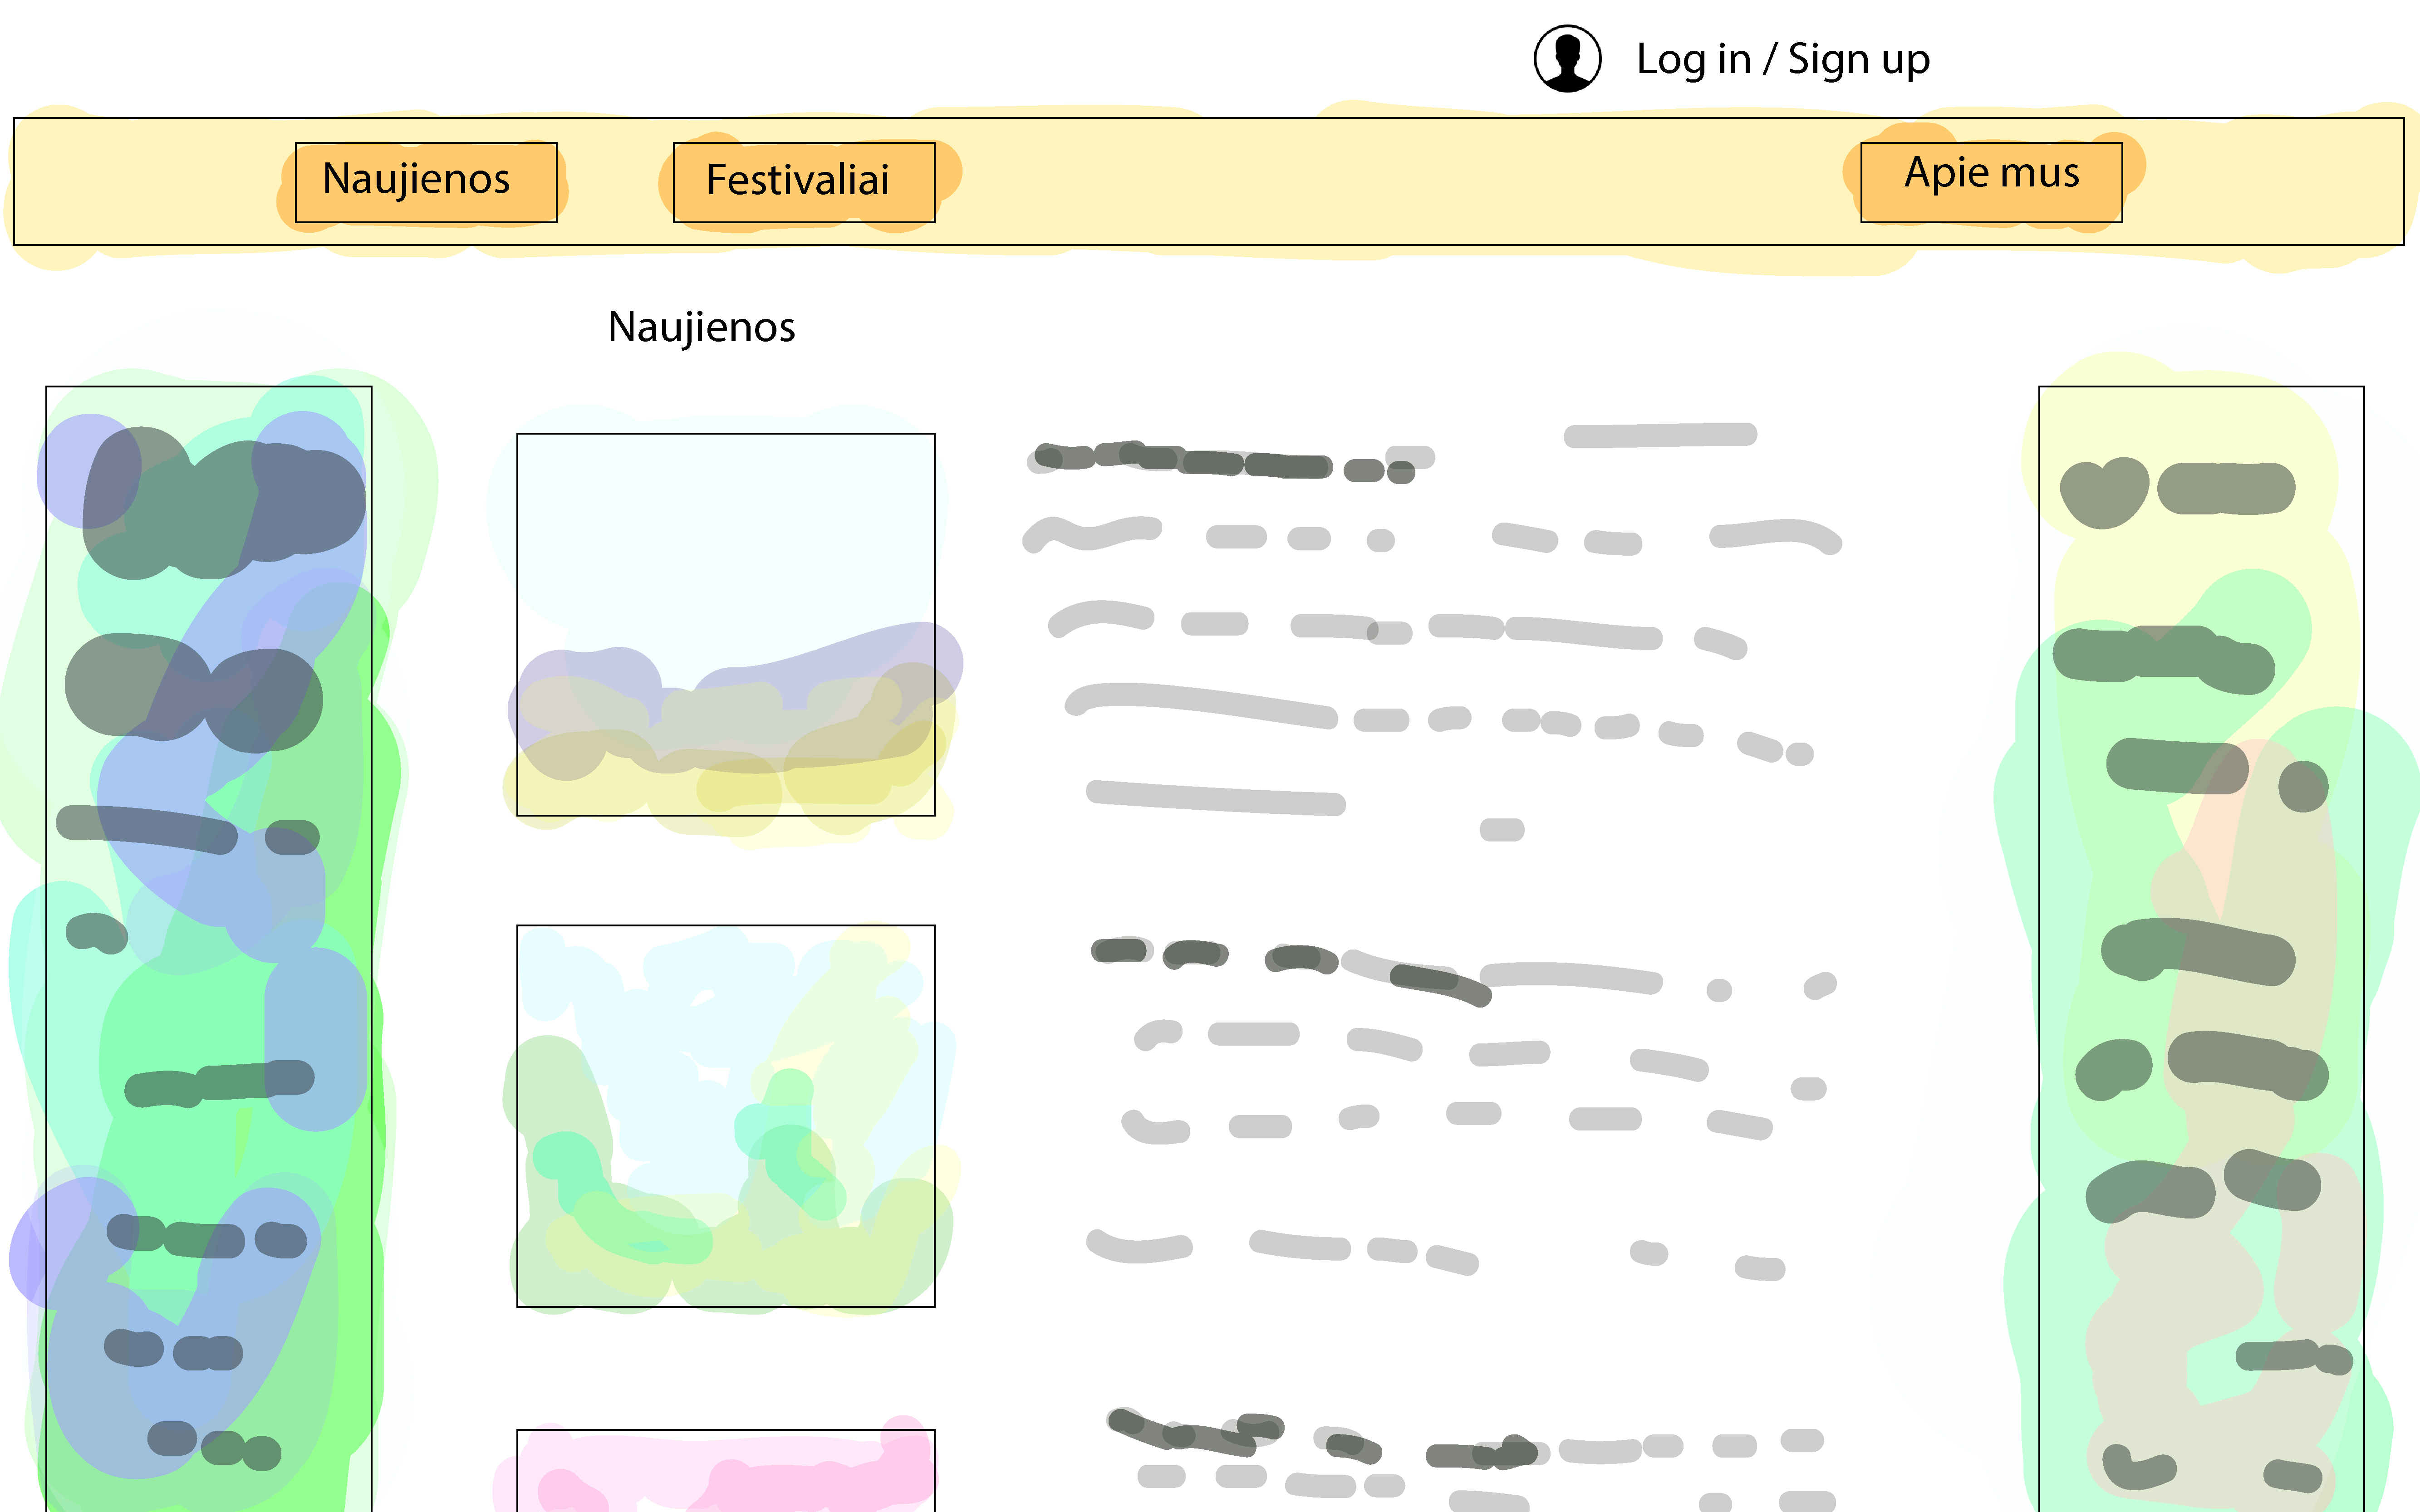
\includegraphics[scale=0.35]{img/PSI2priedai/pirmas-01.jpg}
    \label{img:page1}
	\caption{Festivalių informacijos puslapio eskizas}
\end{figure}

\section{Straipsnių apie festivalius eskizas}
\begin{figure}[H]
    \centering
    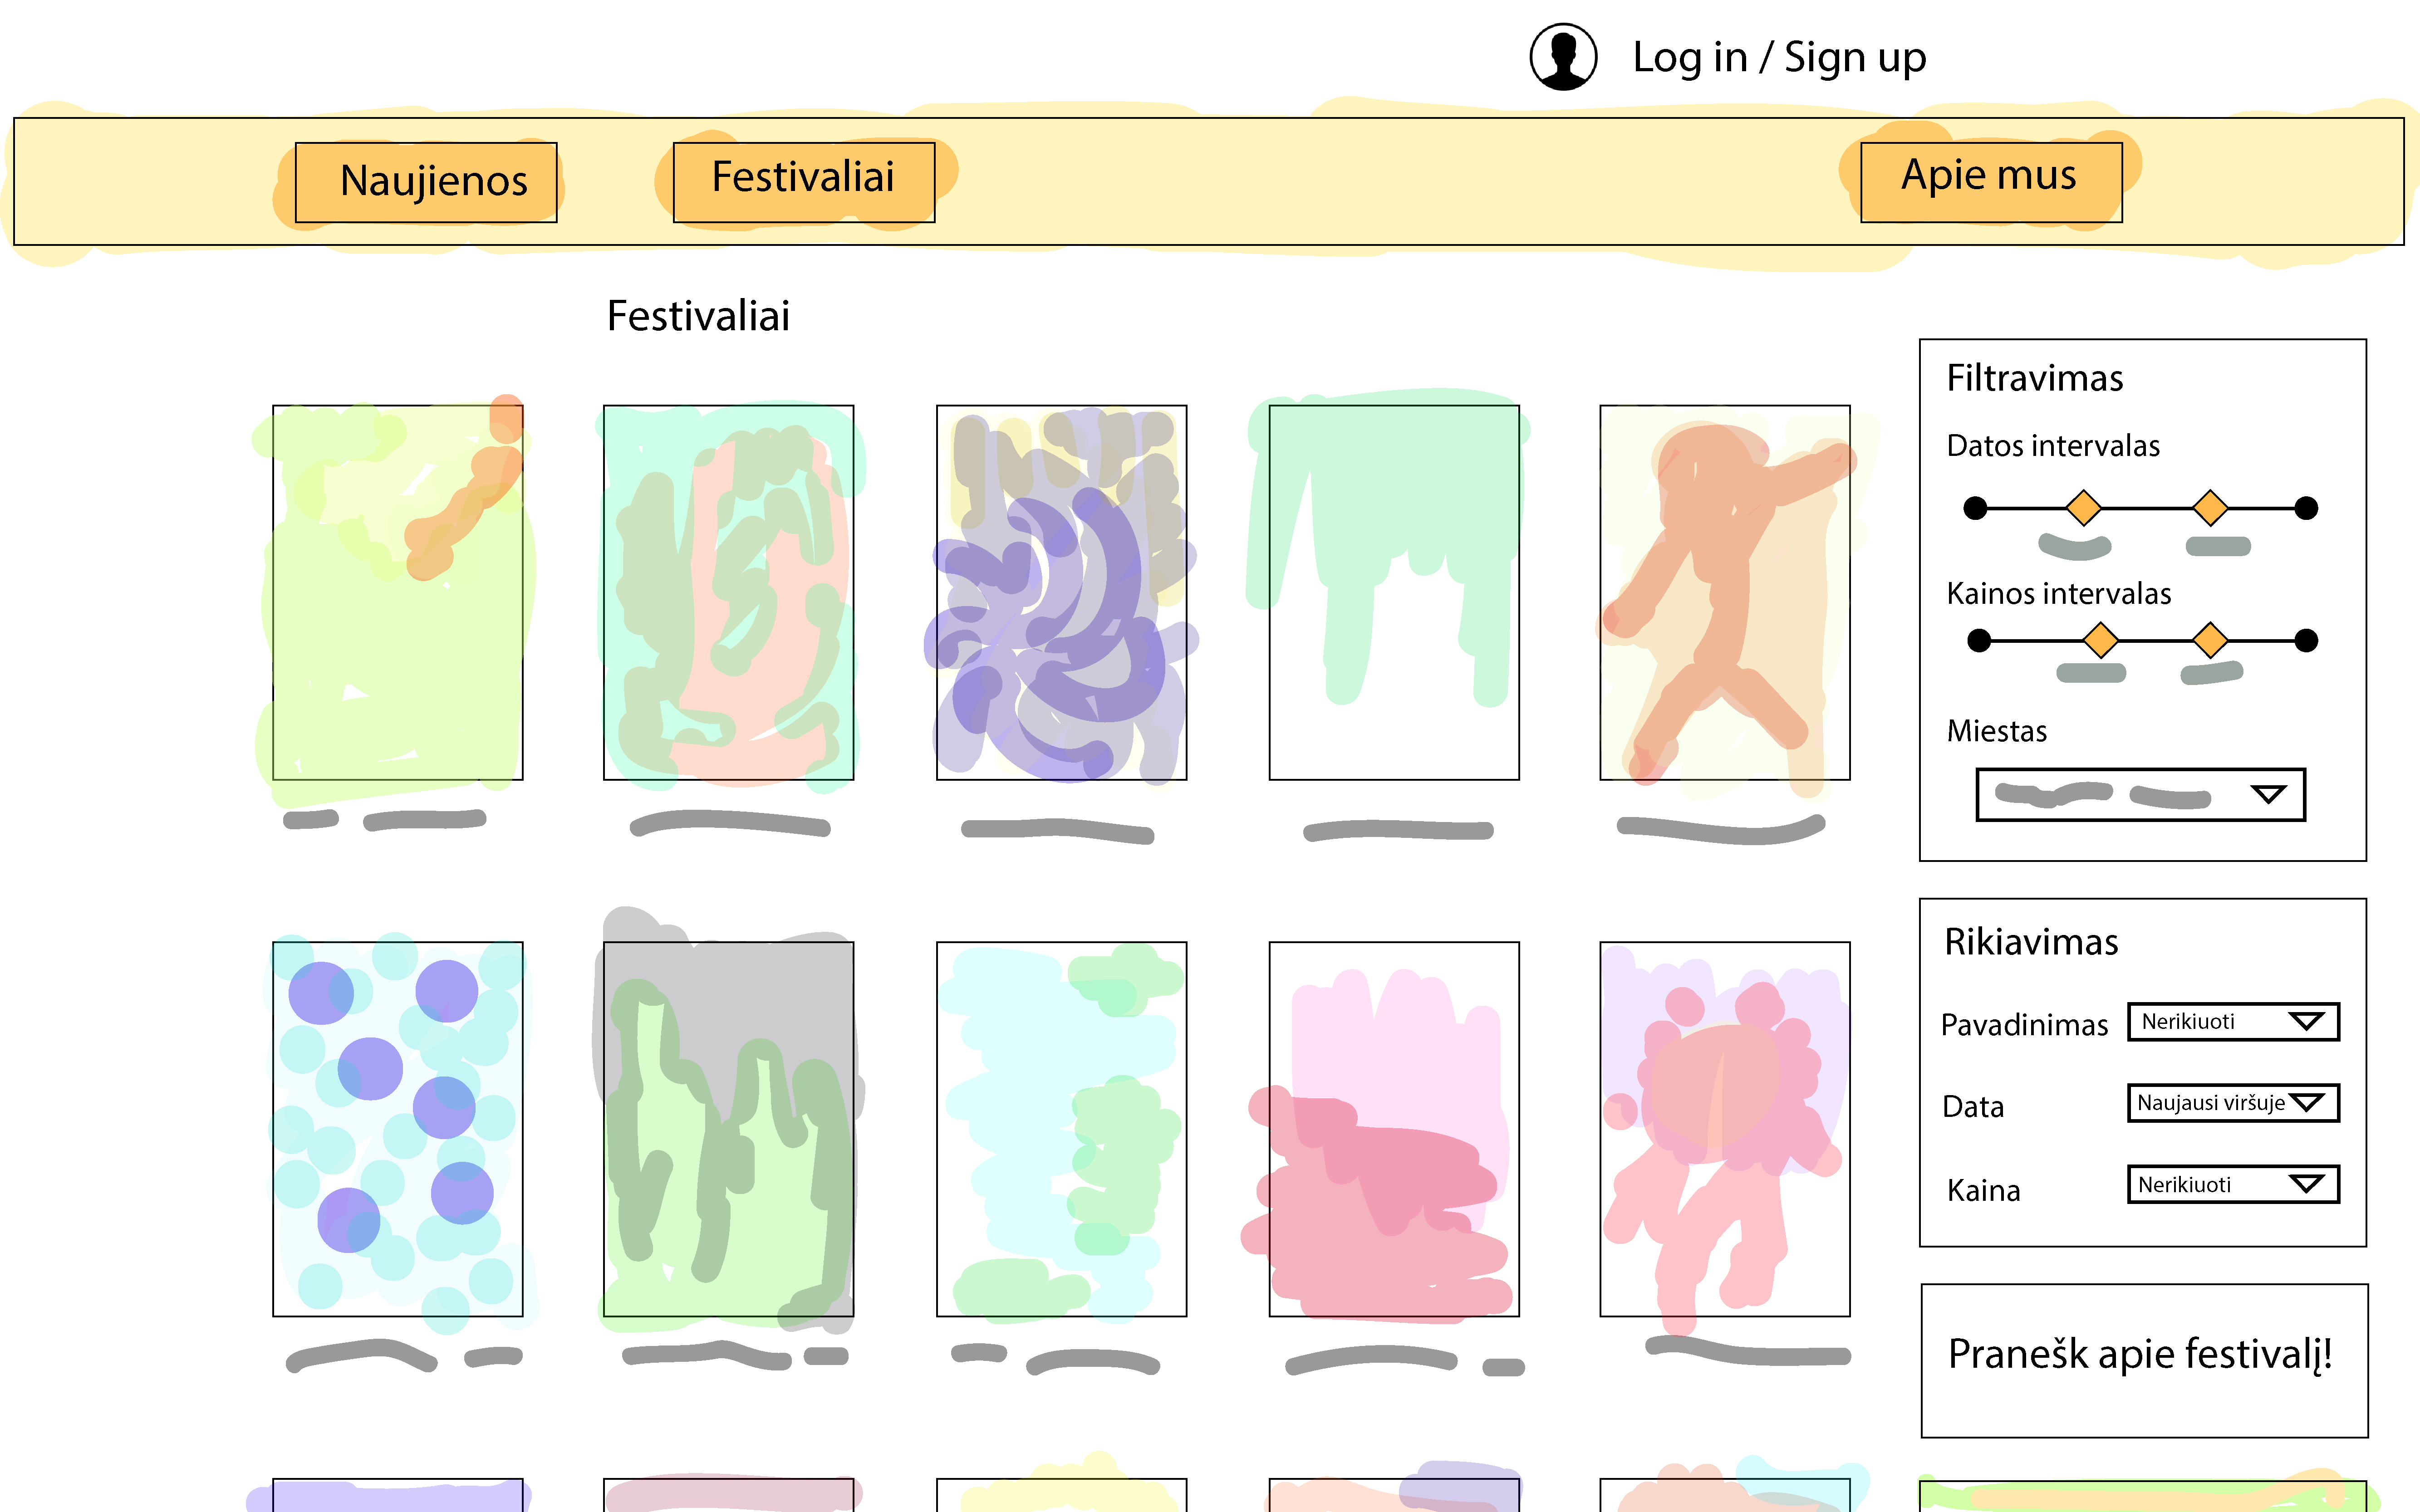
\includegraphics[scale=0.35]{img/PSI2priedai/antras-01.jpg}
    \label{img:page2}
	\caption{Festivalių straipsnių puslapio eskizas}
\end{figure}

\section{Festivalių informacijos puslapio naktinis režimas}
\begin{figure}[H]
    \centering
    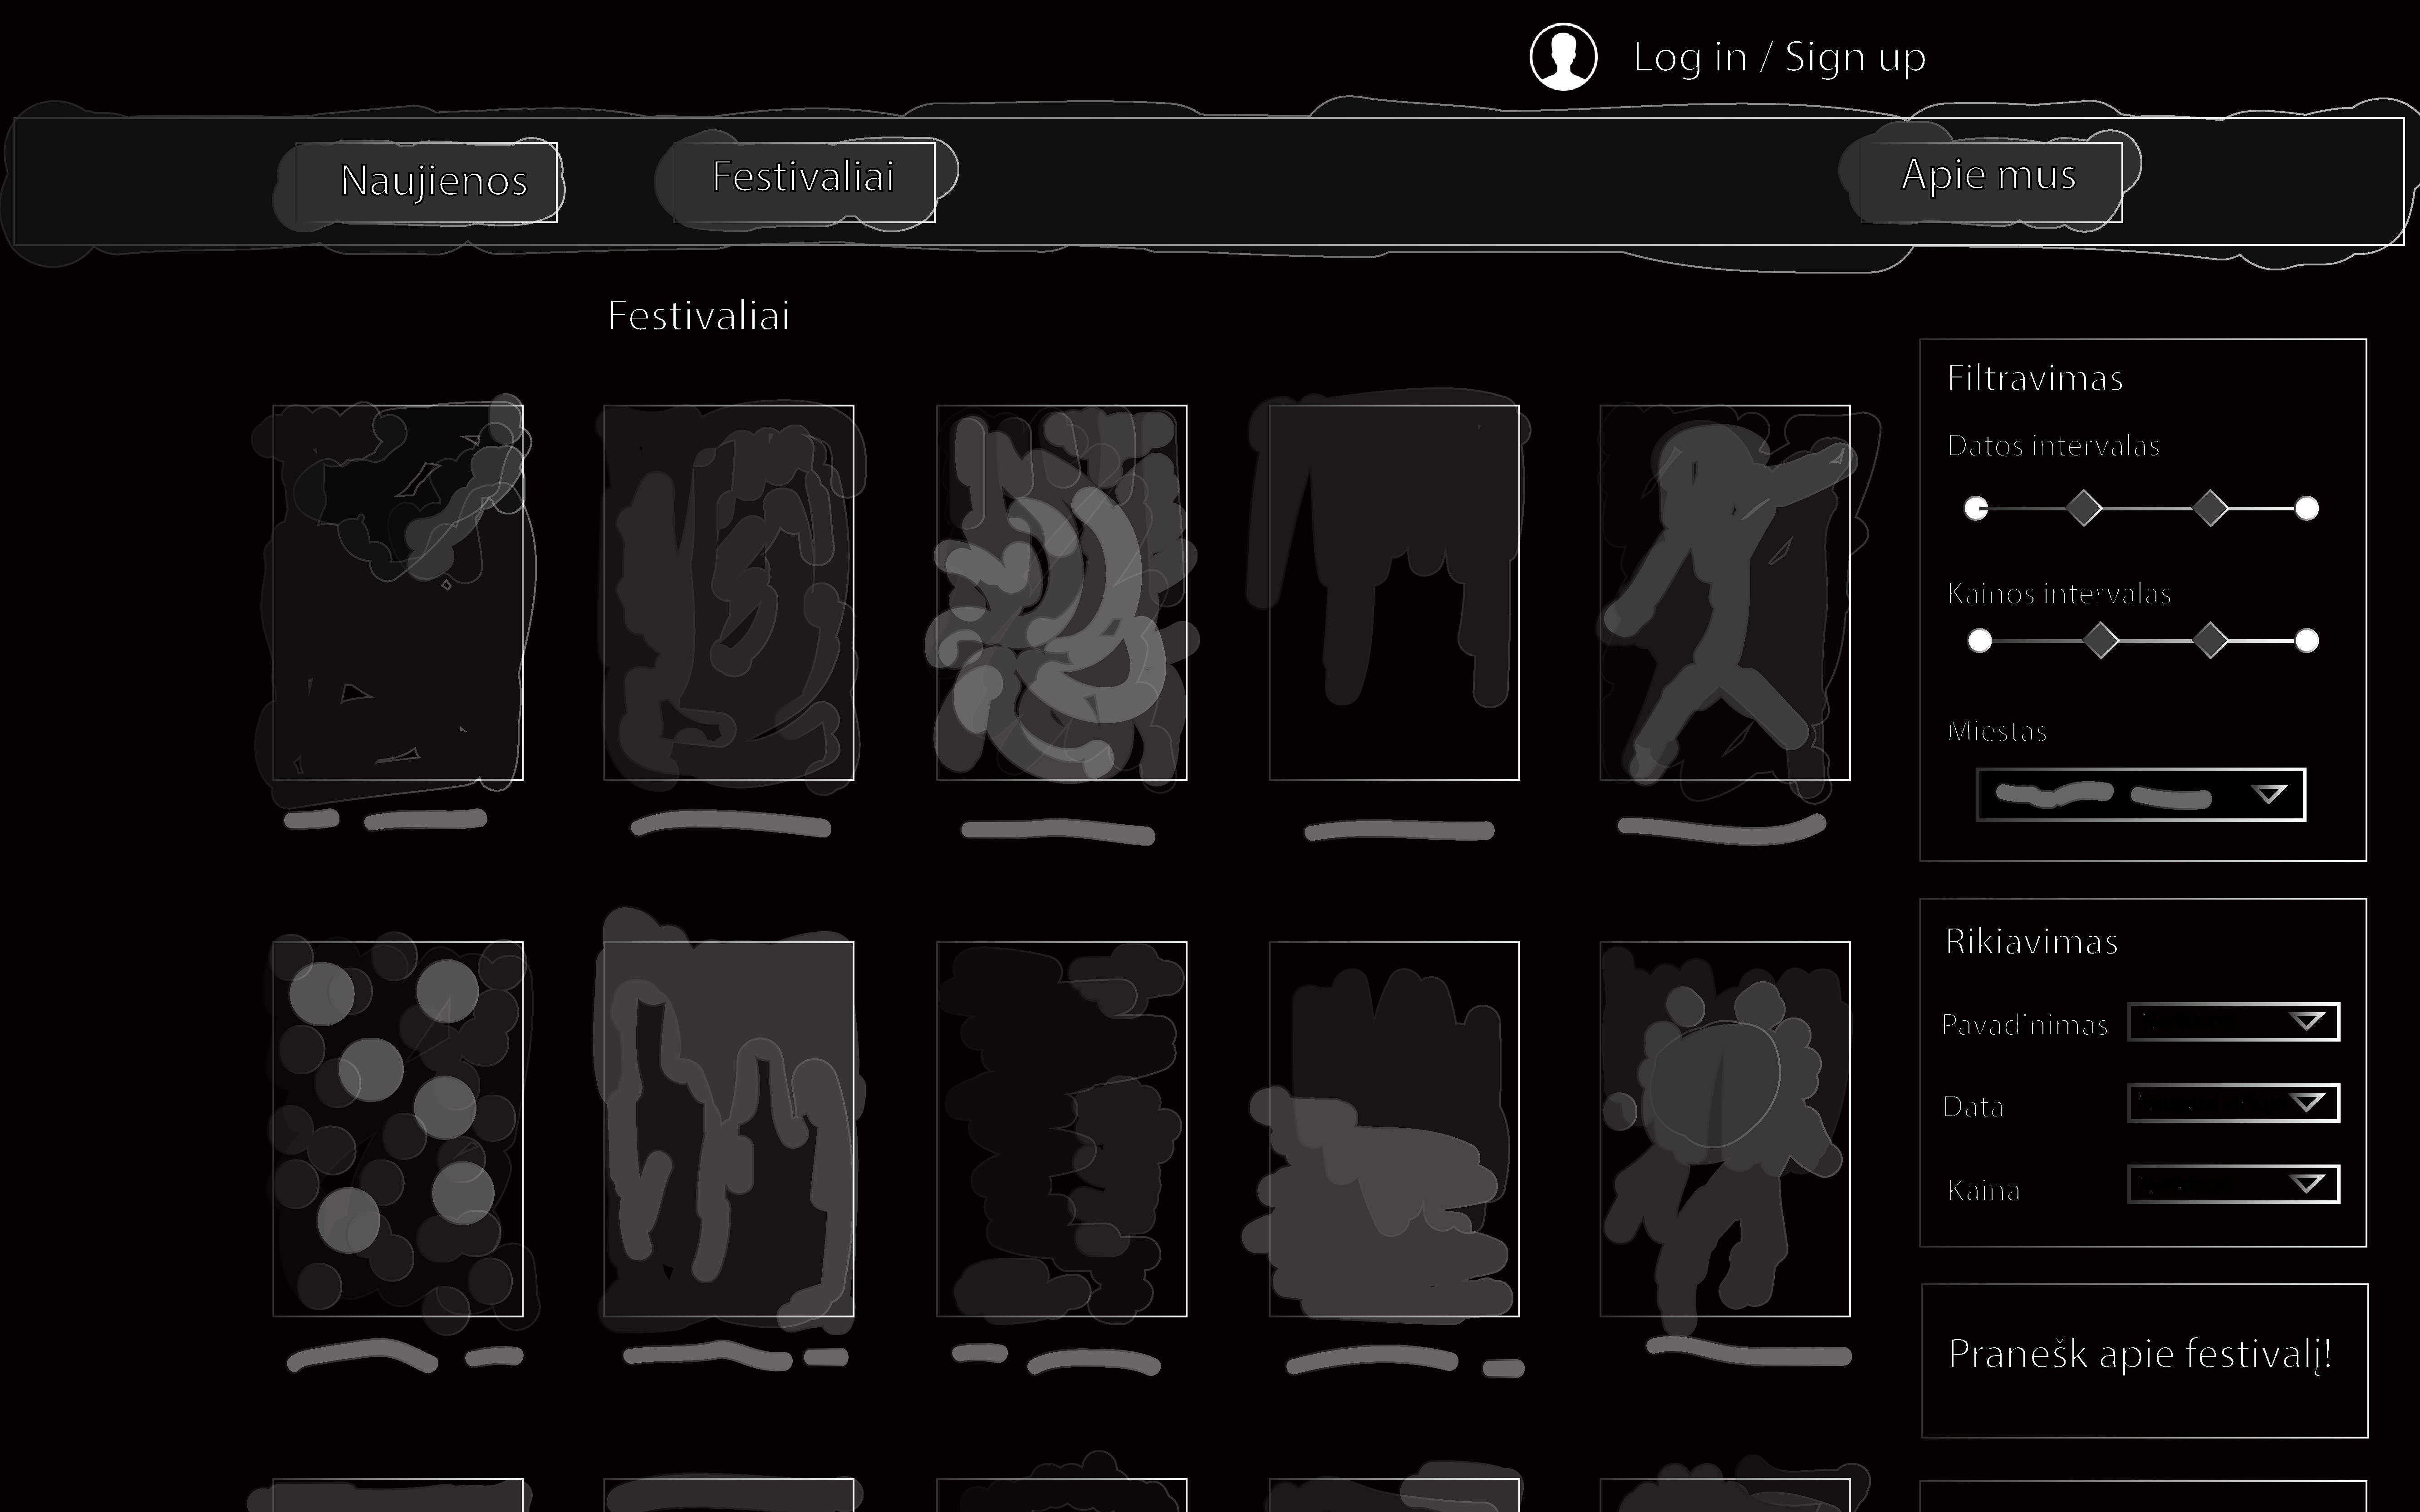
\includegraphics[scale=0.35]{img/PSI2priedai/blackedition.jpg}
    \label{img:page3}
	\caption{Naktionio režimo eskizas}
\end{figure}

% Prieduose gali būti pateikiama pagalbinė, ypač darbo autoriaus savarankiškai
% parengta, medžiaga. Savarankiški priedai gali būti pateikiami ir
% kompaktiniame diske. Priedai taip pat numeruojami ir vadinami. Darbo tekstas
% su priedais susiejamas nuorodomis.

%Citavimo pavyzdžiai: cituojamas vienas šaltinis \cite{PvzStraipsnLt}; cituojami
%keli šaltiniai \cite{PvzStraipsnEn, PvzKonfLt, PvzKonfEn, PvzKnygLt, PvzKnygEn,
%PvzElPubLt, PvzElPubEn, PvzMagistrLt, PvzPhdEn}.
%
%
%\subsubsection{Skirsnis}
%\subsubsubsection{Straipsnis}
%\subsubsection{Skirsnis}%

Pastaba: priedai, kuriuose vaizduojama grafinė vartotojo sąsają, nėra galutiniai - tai tik preliminarūs būsimo tinklalapio kelių puslapių vaizdas.


\end{document}
